\documentclass[11pt,letterpaper]{article}
\usepackage[margin=1in]{geometry}
\usepackage[T1]{fontenc}
\usepackage{lmodern}
\usepackage{amsmath,amssymb,booktabs,array}
\usepackage{graphicx,float}
\usepackage[section]{placeins}
\usepackage[font=small,labelfont=bf]{caption}
\usepackage[numbers,sort&compress]{natbib}
\usepackage[dvipsnames]{xcolor}
\usepackage[colorlinks=true,allcolors=blue]{hyperref}
\usepackage{microtype}
\hypersetup{pdftitle={Intermittency, period adding and bifurcation curves in a language model's own inference map},
  pdfsubject={Private working draft, 12 October 2026}}
\graphicspath{{figures/}}
% Placeholders: red = planned, not started; orange = running or partly done. Remove all before submission.
\newcommand{\planned}[1]{\textcolor{red}{\textbf{[Planned:} #1\textbf{]}}}
\newcommand{\inprogress}[1]{\textcolor{orange}{\textbf{[In progress:} #1\textbf{]}}}
\newcommand{\eps}{\varepsilon}

\title{Intermittency, period adding and bifurcation curves\\ in a language model's own inference map}
\author{Authorship to be decided by the human researcher}
\date{Private working draft, 12 October 2026}

\begin{document}
\maketitle
\noindent\textbf{Status of this draft.} Results without a marker are numerically validated in float64 (evidence
rung 1 or 2 in the sense of Section~\ref{sec:evidence}); \planned{red} marks planned work and
\inprogress{orange} marks running work. Nothing here is a computer-assisted proof yet.

\begin{abstract}
A frozen language model defines its own iterated map when its expected next-token embedding is fed back as
the next input. For Qwen2.5-0.5B-Instruct with a fixed chat prefix, a one-token window, sampling temperature
$T$ and an activation-steering strength $\alpha$, this map of $\mathbb{R}^{896}$ is smooth, and we treat it
with the tools of numerical bifurcation theory. Its $(\log_{10} T,\alpha)$ plane contains deterministic chaos
with embedded periodic windows. A family of windows of periods $6, 8, 10, \dots$ (up to 32 in the maps) reads
as text ``. This'' followed by $k$ pairs ``is X''. The windows accumulate on the fold of the 2-cycle ``is it''
as $\alpha_N-\alpha_c\propto N^{-2}$, where $N$ counts the laps of the ``is it'' loop. We compute the
saddle-node normal form of that fold from derivatives of the network. Without any fitted parameter, it
predicts bottleneck passages of 7 to 144 iterates within one iterate. Natural trajectories re-enter the
bottleneck near its middle, which fixes the prefactor of the window law. This is type-I intermittency
(Pomeau--Manneville) inside the inference computation of a pretrained language model. We continue fold and
flip curves of the periodic orbits with float64 test functions. In a higher-temperature region we find a
fold curve with two cusps whose normal-form coefficient changes sign, the codimension-two organization of
shrimp-shaped windows. Replacing the expected embedding by averages of $m$ sampled embeddings shows how much
of the mechanism survives sampling. A recurrent-depth model (Huginn-0125) gives a second system, in which a
Neimark--Sacker bifurcation predicted from the spectrum of the native fixed point appears where predicted.
\planned{replication across prompts, steering directions and model sizes; one-sentence summary of it.}
\end{abstract}

\section{Introduction}
\label{sec:intro}
Repeated inference with a fixed language model is an iterated map: the model's output becomes its next input.
Recent work has measured chaos-like sensitivity in language-model generation
\cite{li2025quasilyapunov,jaca2026chaos}, temperature-driven changes of output statistics
\cite{arnold2024phase,nakaishi2024phase,sun2025phase,ruan2026criticality,johnson2026temperature}, periodic
attractors of paraphrasing loops \cite{wang2025attractor}, attractor states of model-to-model conversations
\cite{ko2026attractor}, and the stability of looped and recurrent-depth models through their Jacobians
\cite{bai2019deq,bai2021stabilizing,tomihari2025recurrent,yang2026stars,luo2026prediction}. Feeding a
probability-weighted vocabulary embedding back into a model is itself not new \cite{zeng2025ponderlm}, nor is
continuous latent feedback \cite{hao2024coconut}.

What these studies do not do is resolve the invariant sets of an exactly defined inference map and the
bifurcations that organize them. We do that for one constructed but exact system, the expected-embedding
(``soft-token'') map of a frozen pretrained model. It is smooth, its Jacobians are available by automatic
differentiation, and its periodic orbits can be computed and continued like those of any smooth map. The
emphasis is quantitative: a local normal form computed from the network's derivatives predicts a long-time
observable without fitting.

\paragraph{Contributions.}
\begin{enumerate}
\item Phase maps of the soft-token map in temperature and steering strength, in float64, showing chaos with
  embedded periodic windows (Section~\ref{sec:maps}).
\item A period-adding family of primitive periodic orbits whose text adds one ``is X'' pair per period step,
  with multipliers from the monodromy matrix (Section~\ref{sec:adding}).
\item The mechanism: the 2-cycle ``is it'' dies in a fold; its normal form, computed from derivatives, predicts
  bottleneck passage times; the global reinjection sets the window-law prefactor (Section~\ref{sec:mechanism}).
\item Fold and flip curves of periodic orbits continued in the parameter plane with float64 test functions,
  including two cusps on a period-4 fold curve (Section~\ref{sec:curves}).
\item A bridge to sampled decoding (Section~\ref{sec:bridge}) and a second system, a recurrent-depth model with
  a predicted and observed Neimark--Sacker bifurcation (Section~\ref{sec:huginn}).
\end{enumerate}
\planned{related-work section from the systematic literature search (Codex task 3); keep the boundaries drawn
in the two prior-work reviews.}

\section{The inference map}
\label{sec:map}
\paragraph{Definition.} Let $E\in\mathbb{R}^{V\times d}$ be the input embedding matrix ($V=151{,}936$,
$d=896$) and let $z(x)\in\mathbb{R}^V$ be the next-token logits produced by the model, given a fixed chat prefix
(system prompt ``You are an AI talking with another AI. You have complete freedom. Feel free to pursue whatever
you want.'' and user turn ``Hello!'') followed by a single input embedding $x$. The soft-token map is
\begin{equation}
  F_{T,\alpha}(x) = E^{\top}\operatorname{softmax}\!\big(z_\alpha(x)/T\big),
\end{equation}
where $z_\alpha$ adds $\alpha v$ to the residual stream at layer 12 at every position, prefix included, and $v$
is a contrastive steering direction (``philosophy'' prompts against neutral prompts, last-token states,
normalized to the mean residual norm). Positions are fixed (the window does not grow), so $F$ is an autonomous
map of $\mathbb{R}^{896}$. As $T\to0$ it reduces to greedy decoding of the same fixed-prefix, one-token-window
system when the argmax is unique; it is not ordinary generation with a growing context.

\paragraph{Precision.} Hugging Face RMSNorm and rotary-embedding tables compute in float32 even when the model is
cast to float64; we patch both. float32 maps are accurate to $3\times10^{-6}$--$2\times10^{-5}$ per step, which is
enough for phase maps (245 of 256 test cells agree with float64) but not for derivatives of composed maps:
one-step float32 Jacobian-vector products are accurate to $5\times10^{-5}$, yet the 8-step monodromy of a
period-8 orbit is off by 3\%. All orbits, multipliers and test functions below are float64.

\section{Methods}
\label{sec:methods}
\paragraph{Phase maps.} For each cell, 300 transient and 300 measured steps; the largest Lyapunov exponent from a
renormalized twin at offset $10^{-6}$; the period as the smallest $q\le32$ with return distance below
$10^{-8}$; the attractor's identity as its rotation-invariant leading-token loop. Maps of $256^2$ cells take
about 100 minutes on one H100 GPU in float64.
\paragraph{Periodic orbits.} Newton's method on $F^p(x)-x$ with forward-mode Jacobians; multipliers are the
eigenvalues of the monodromy matrix, refined by a short Arnoldi factorization with float64 Jacobian-vector
products where the dense matrix is not float64.
\paragraph{Continuation.} Pseudo-arclength continuation of periodic branches in one parameter, and of fold and
flip curves in two, using minimally augmented systems \cite{govaerts2000numerical,kuznetsov2023elements}: the
test function $g$ of the bordered system $[[M\mp I,b],[c^\top,0]]$ is obtained by GMRES with Jacobian-vector
products, and its gradient by reverse-mode differentiation through a Jacobian-vector product. A reversal of the
parameter tangent flags a cusp candidate, which we test with the normal form.
\paragraph{Normal form and passages.} For the two-step map $G=F^2$ at a fold with right and left eigenvectors
$r,\ell$ ($\|r\|=1$, $\ell^\top r=1$), $u'=u+a\eps+bu^2$ with $a=\ell^\top\partial_\alpha G$ and
$b=\tfrac12\ell^\top D^2G[r,r]$; $b$ is computed by central differences of float64 Jacobian-vector products over
a step-size plateau, and $a$ includes the steering's effect on the prefix. Passage counts are compared with the
iterated quadratic map and with the arctangent formula \cite{pomeau1980intermittent}.

\section{Chaos with periodic windows}
\label{sec:maps}
Figure~\ref{fig:stripes} shows a $256\times256$ float64 map over $\alpha\in[0.060,0.082]$,
$\log_{10}T\in[-0.17,-0.04]$: 35{,}759 of 65{,}536 cells are chaotic, and periodic windows of periods 2--32 are
embedded among them. Rendered as in the shrimp literature \cite{stenzinger2025shrimp}, periodic regions show
dark curves of maximal contraction inside the windows.
\begin{figure}[H]
\centering
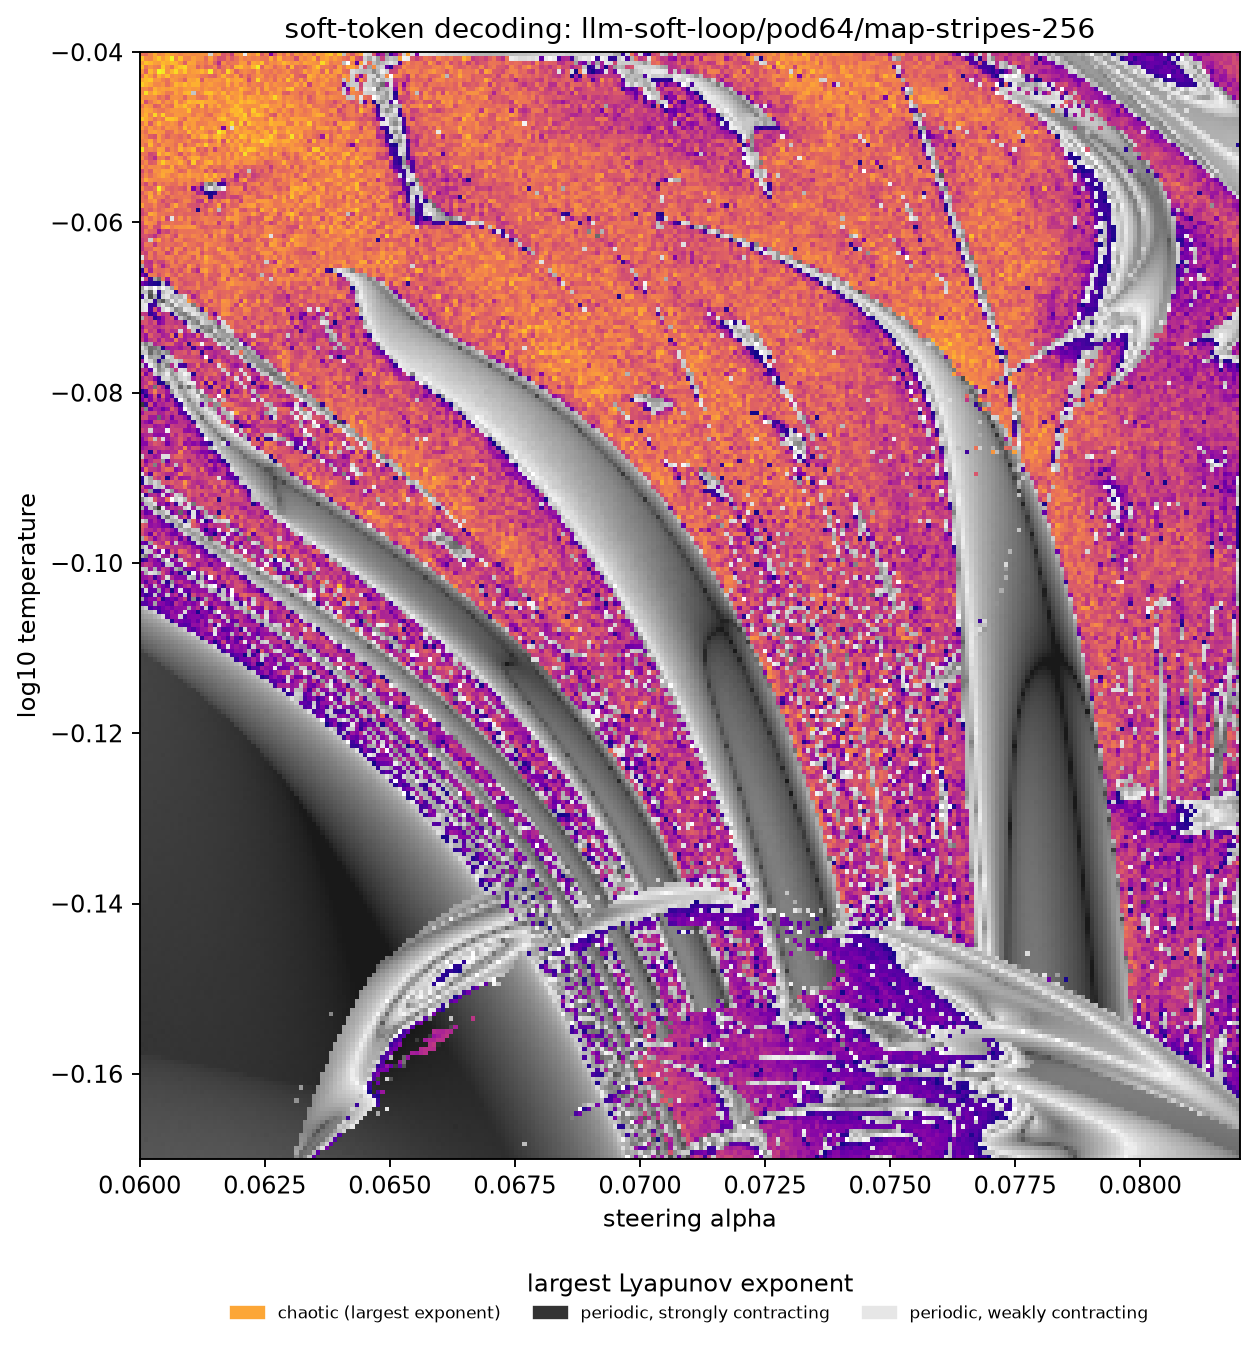
\includegraphics[width=0.49\linewidth]{fig-stripes-lyapunov.png}\hfill
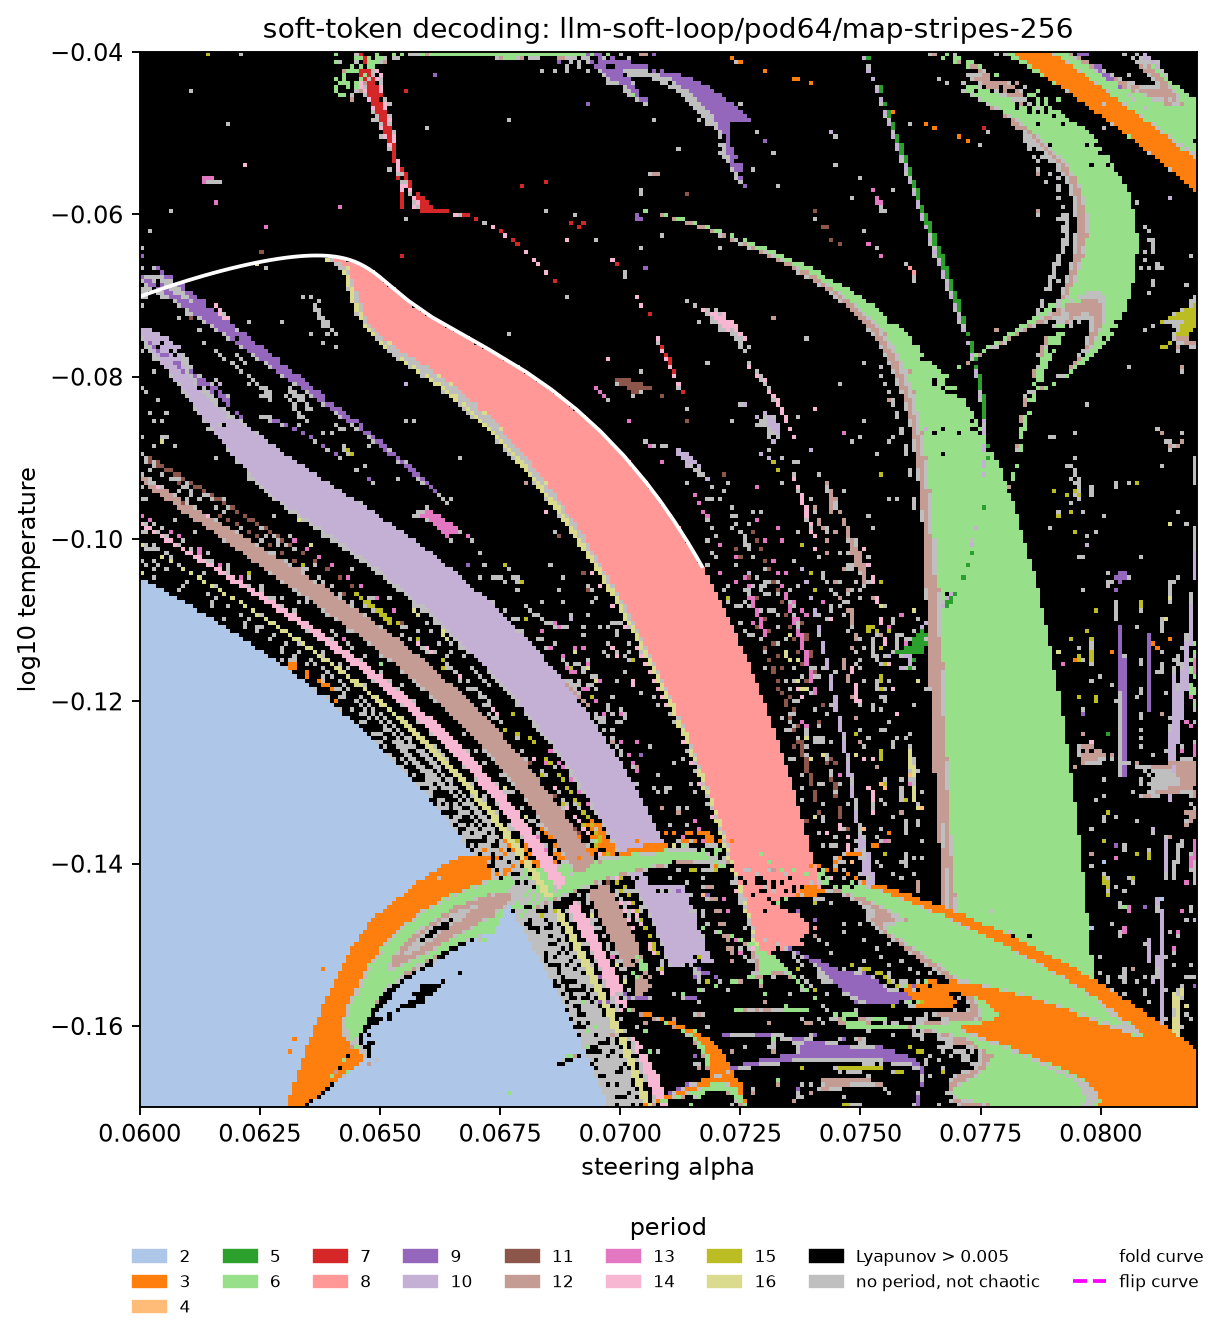
\includegraphics[width=0.49\linewidth]{fig-stripes-period-fold.png}
\caption{Soft-token map of Qwen2.5-0.5B, $256^2$ float64 cells. Left: chaotic cells coloured by the largest
Lyapunov exponent, periodic cells in grey by how strongly they contract. Right: periods; the white curve is the
continued fold curve of the period-8 orbit (Section~\ref{sec:curves}).}
\label{fig:stripes}
\end{figure}
\inprogress{$512^2$ float64 map of the stripes' lower ends and the crossing bands (four bands running); three
$256^2$ zooms with attractor identities; nested-zoom figure.}

\section{Period adding written in text}
\label{sec:adding}
Between a period-2 region and the chaos lies a fan of stripes of periods $6, 8, 10, \dots$ Their orbits,
numerically validated in float64 (Newton residuals $10^{-13}$--$10^{-15}$), read as text
(Table~\ref{tab:orbits}): ``. This'' followed by $k$ pairs ``is X'', period $2k+2$. The period-2 region is the
2-cycle ``is it''. The multipliers are effectively one-dimensional: one is of order $10^{-3}$--$10^{-1}$, all
others of order $10^{-6}$.
\begin{table}[H]
\centering\small
\begin{tabular}{rlll}
\toprule
period & leading tokens of the orbit & $(\log_{10}T,\alpha)$ & leading multiplier \\
\midrule
2 & is it & $(-0.1726, 0.0616)$ & $-0.27$ \\
6 & . This is a is a & $(-0.1205, 0.0786)$ & \planned{float64 value} \\
8 & . This is there is a is a & $(-0.1205, 0.0717)$ & $+0.0041$ \\
10 & . This is there is it is a is a & $(-0.1089, 0.0673)$ & $+0.0024$ \\
12 & . This is it is it is it is a is a & $(-0.1090, 0.0641)$ & $+0.072$ \\
\bottomrule
\end{tabular}
\caption{Periodic orbits of the stripe family. \planned{Recompute all rows with today's float64 map (patched
rotary tables) and add periods 14--20.}}
\label{tab:orbits}
\end{table}

\section{Mechanism: a saddle-node bottleneck}
\label{sec:mechanism}
\paragraph{The fold.} At $\log_{10}T=-0.115$ the 2-cycle ``is it'' dies in a fold at $\alpha_c=0.06279827$ (float64
multiplier $1$ to $3\times10^{-13}$, other multipliers below $0.04$). The normal form of $G$ has $a=-4.834$ per
unit $\alpha$ and $b=-25.4285$, so $ab=122.93$; extrapolating the stable-branch multipliers,
$(1-\mu)^2/(4(\alpha_c-\alpha))\to ab$, gives $123.1$ independently.

\paragraph{Controlled passages.} Starting at $u_{\rm in}=-U$ or $0$ ($U=0.1/|b|$) and counting $G$-iterates until
$u>U$, the measured counts match the iterated normal form within one iterate at four held-out distances
(Table~\ref{tab:passages}, Figure~\ref{fig:passages}); a transverse displacement of the same norm changes the
count by at most one.
\begin{table}[H]
\centering\small
\begin{tabular}{rcccc}
\toprule
$\eps=\alpha-\alpha_c$ & full: measured / predicted & midpoint & full + transverse kick \\
\midrule
$3\times10^{-6}$ & 144 / 144 & 73 / 74 & 143 / 144 \\
$1\times10^{-5}$ & 71 / 71 & 36 / 37 & 70 / 71 \\
$3\times10^{-5}$ & 34 / 34 & 17 / 18 & 33 / 34 \\
$1\times10^{-4}$ & 14 / 14 & 7 / 7 & 13 / 14 \\
\bottomrule
\end{tabular}
\caption{Bottleneck passages ($G$-iterates). Predictions iterate $u'=u+a\eps+bu^2$ with $a,b$ computed from the
network's derivatives; no parameter is fitted.}
\label{tab:passages}
\end{table}
\begin{figure}[H]
\centering
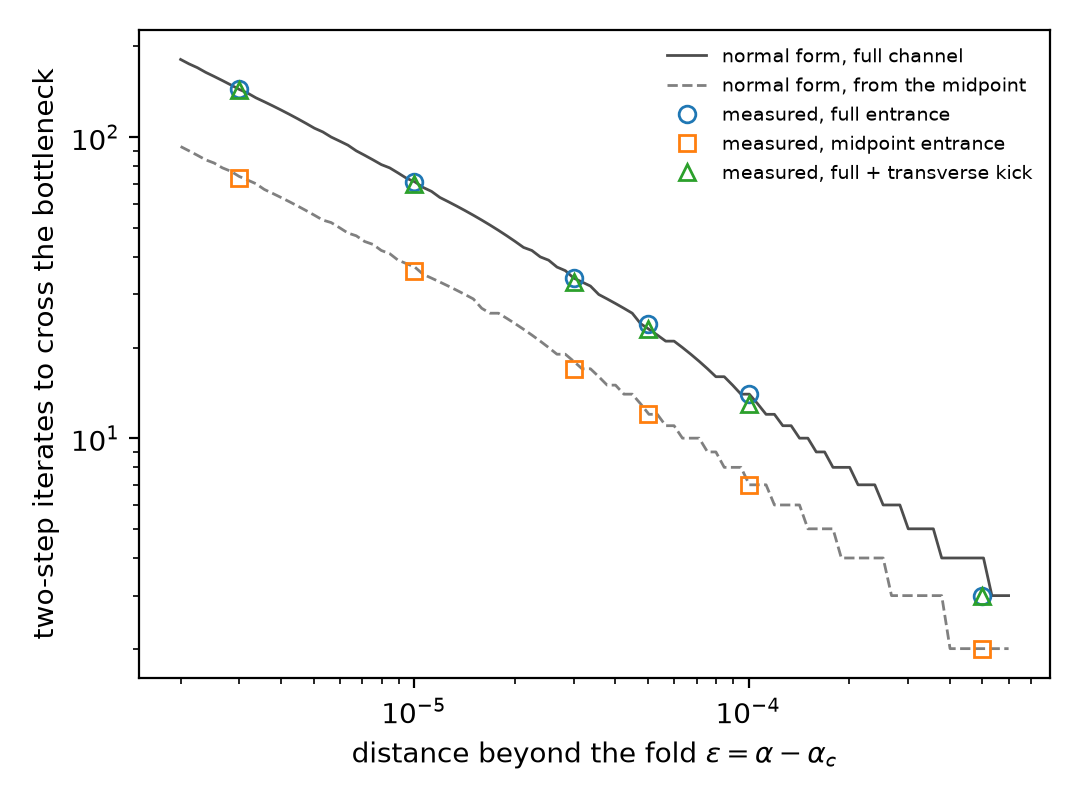
\includegraphics[width=0.49\linewidth]{fig-passages.png}\hfill
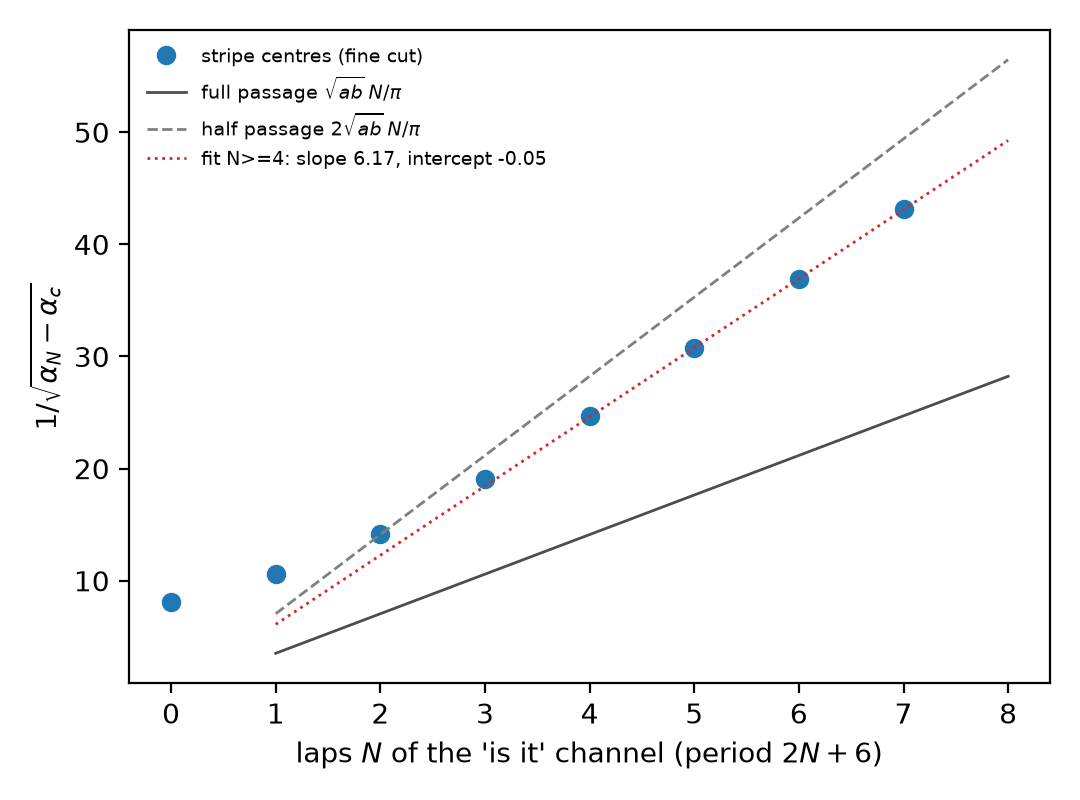
\includegraphics[width=0.49\linewidth]{fig-window-law.png}
\caption{Left: passage times against the normal-form predictions. Right: window law; stripe centres
$1/\sqrt{\alpha_N-\alpha_c}$ against the lap count $N$, with the full- and half-passage predictions.}
\label{fig:passages}
\end{figure}

\paragraph{Natural reinjection and the window law.} Free trajectories re-enter the channel slightly upstream of
the bottleneck's middle ($u\approx-3\times10^{-4}$ to $-7\times10^{-4}$). From each measured entry point the
normal form predicts the natural laminar durations within 4--8\% for $\eps\le10^{-4}$, and a natural passage lasts
about 0.6 of a full one. The stripes therefore follow the $N^{-2}$ law of a saddle-node ghost with about a third
of the full-passage prefactor: stripe centres give $d_N N^2=0.0263$--$0.0265$ for $N=4$--$7$ (log-log slope
$-2.00$), compared with $\pi^2/(4ab)=0.0201$ for a half passage. Two-step return maps of $p(\text{``it''})$
(Figure~\ref{fig:returnmaps}) show the near-tangency.
\inprogress{stripe edges from continuation (ladder of branches for periods 6--20) instead of grid-defined
centres; prediction of the window positions from the measured reinjection distribution.}
\begin{figure}[H]
\centering
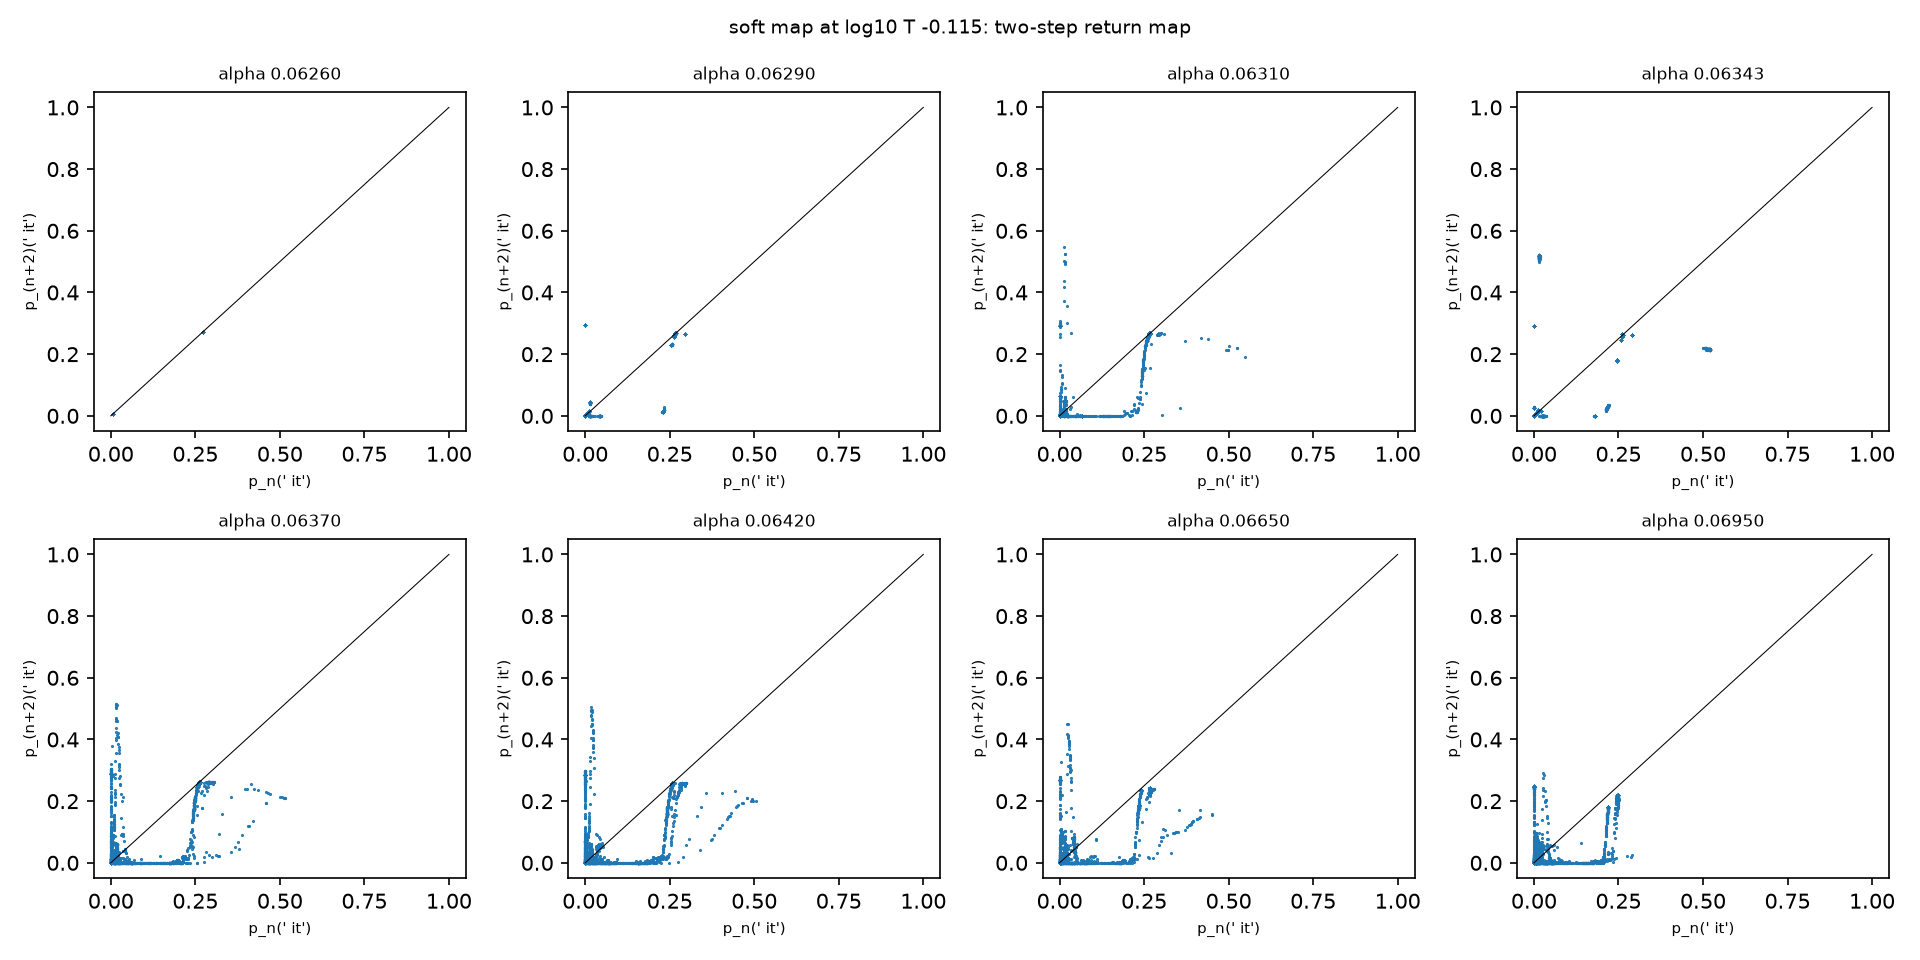
\includegraphics[width=0.85\linewidth]{fig-return-maps.png}
\caption{Two-step return maps of the probability of ``it'' near the 2-cycle's fold, at increasing distance from
it.}
\label{fig:returnmaps}
\end{figure}

\section{Bifurcation curves and cusps}
\label{sec:curves}
\paragraph{Period-8 stripe.} The fold curve of the period-8 orbit, continued for 80 points with a float64 test
function, keeps its critical multiplier within $1\pm6\times10^{-6}$, follows the stripe's upper edge, and caps
its top near $\log_{10}T=-0.065$ (Figure~\ref{fig:stripes}). At $\alpha=0.0717$ the stripe lies between a flip at
$\log_{10}T=-0.128955$ and the fold at $-0.1033462$. \inprogress{flip curve in both directions; fold curve toward
the stripe's lower end; fold curve of the 2-cycle (the accumulation boundary).}

\paragraph{A period-4 window with two cusps.} At higher temperature, $\log_{10}T\approx0$--$0.1$, periodic orbits
are no longer effectively one-dimensional (second multipliers $0.06$--$0.09$). In temperature at
$\alpha=0.06484$ the branch of the period-4 orbit ``$\backslash$n$\backslash$n - $\backslash$n$\backslash$n The''
is S-shaped, with folds at $\log_{10}T=0.0640$ and $0.0664$. Continuing that fold in the plane, its parameter
tangent reverses twice; at both reversals the normal-form coefficient $b$ changes sign while $a$ stays away from
zero (Table~\ref{tab:cusps}), so both are cusps of the fold curve, at $(\alpha,\log_{10}T)=(0.06296,0.05996)$ and
$(0.06557,0.07445)$. Between the two fold branches two period-4 orbits coexist (Figure~\ref{fig:p4}).
\begin{table}[H]
\centering\small
\begin{tabular}{lcc}
\toprule
 & cusp 1 & cusp 2 \\
\midrule
$b$ at five consecutive curve points & $+28.1,\ +18.7,\ +8.4,\ \mathbf{-1.1},\ -12.8$ &
  $+51.8,\ +29.7,\ +9.3,\ \mathbf{-9.0},\ -23.4$ \\
$a$ & $3.02$--$3.08$ & $-2.58$ to $-2.57$ \\
critical multiplier & $1\pm10^{-9}$ & $1\pm10^{-8}$ \\
\bottomrule
\end{tabular}
\caption{Normal-form test of the two parameter-tangent reversals (bold: the flagged points).
\planned{cubic coefficient (nondegeneracy).}}
\label{tab:cusps}
\end{table}
\begin{figure}[H]
\centering
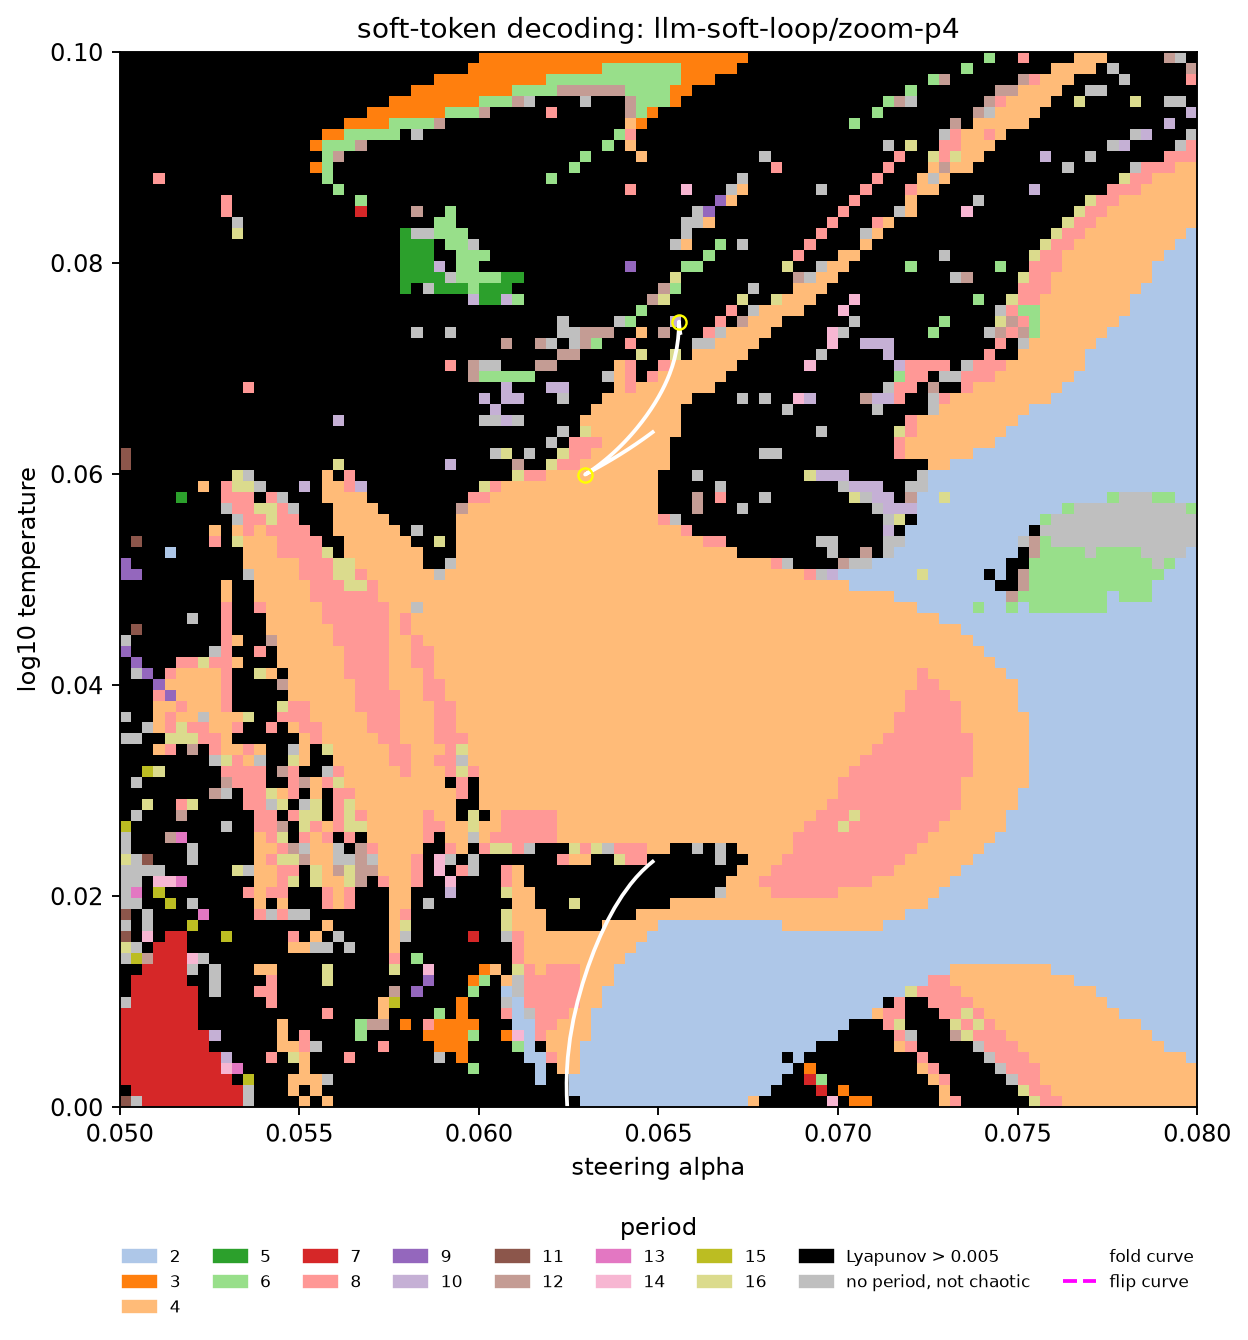
\includegraphics[width=0.6\linewidth]{fig-p4-curves.png}
\caption{Period map of the high-temperature region (float32, $96^2$) with float64 fold curves of the period-4
orbit; yellow circles are the two cusps. \inprogress{float64 $256^2$ map coloured by attractor identity; remaining
fold and flip curves; whether the region is one shrimp-organized component.}}
\label{fig:p4}
\end{figure}
\planned{Codimension-two points where a second multiplier crosses the unit circle along the lower fold curve
(candidate fold-flip points): locate, type and continue.}

\section{Bridge to sampled decoding}
\label{sec:bridge}
Replacing the expected embedding by the mean of $m$ sampled token embeddings (Figure~\ref{fig:bridge}): with the
exact map, laminar phases near the fold last 120 and 63 steps at $\eps=10^{-5}$ and $3\times10^{-5}$; with
$m=64$ they last about 10.6 steps independently of $\eps$ (57\% of steps in the channel); with $m=8$, about 7.7
steps (38\%); with single samples ($m=1$, sampled decoding of the same truncated system) essentially no
laminar phases remain (11\% of steps in the channel). The deterministic intermittency mechanism belongs to the
expected-embedding map; sampling noise turns the bottleneck into a noise-limited trap whose strength grows with $m$.
\begin{figure}[H]
\centering
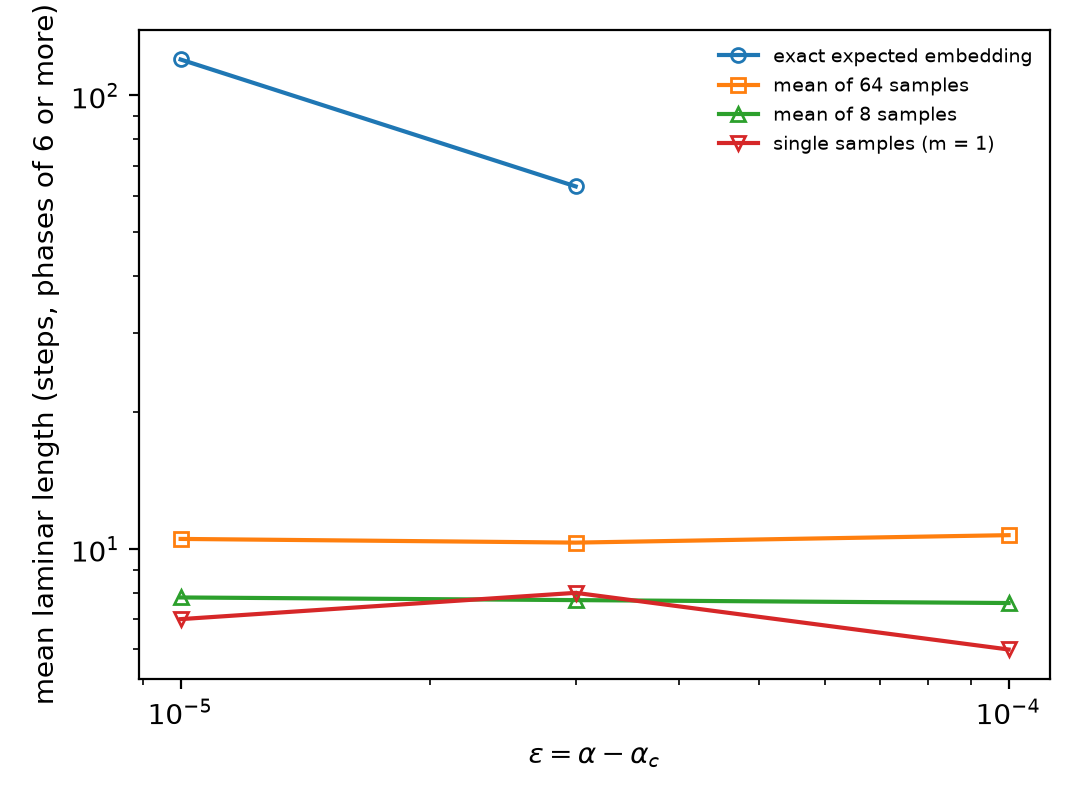
\includegraphics[width=0.55\linewidth]{fig-bridge.png}
\caption{Mean laminar length against $\eps$ for the exact map and for $m$ sampled embeddings.}
\label{fig:bridge}
\end{figure}

\section{Replication and scale}
\label{sec:scale}
For Qwen2.5-1.5B (steering at layer 14 of 28), a coarse $64^2$ float64 map over the same range again shows
chaotic regions with embedded windows of periods up to 32, with different text loops (``!Hello'',
``What?'', ``$\backslash$nWhat is a'') (Figure~\ref{fig:qwen15}).
\inprogress{$256^2$ zoom of the 1.5B chaotic zone (four bands running); search for a fold and stripes; normal-form
passage test.}
\planned{frozen-design replication on fresh prompts and a second steering direction (gratitude); Qwen 7B and one
7--8B model of another family; scaling of $ab$ and of the window law with model size.}
\begin{figure}[H]
\centering
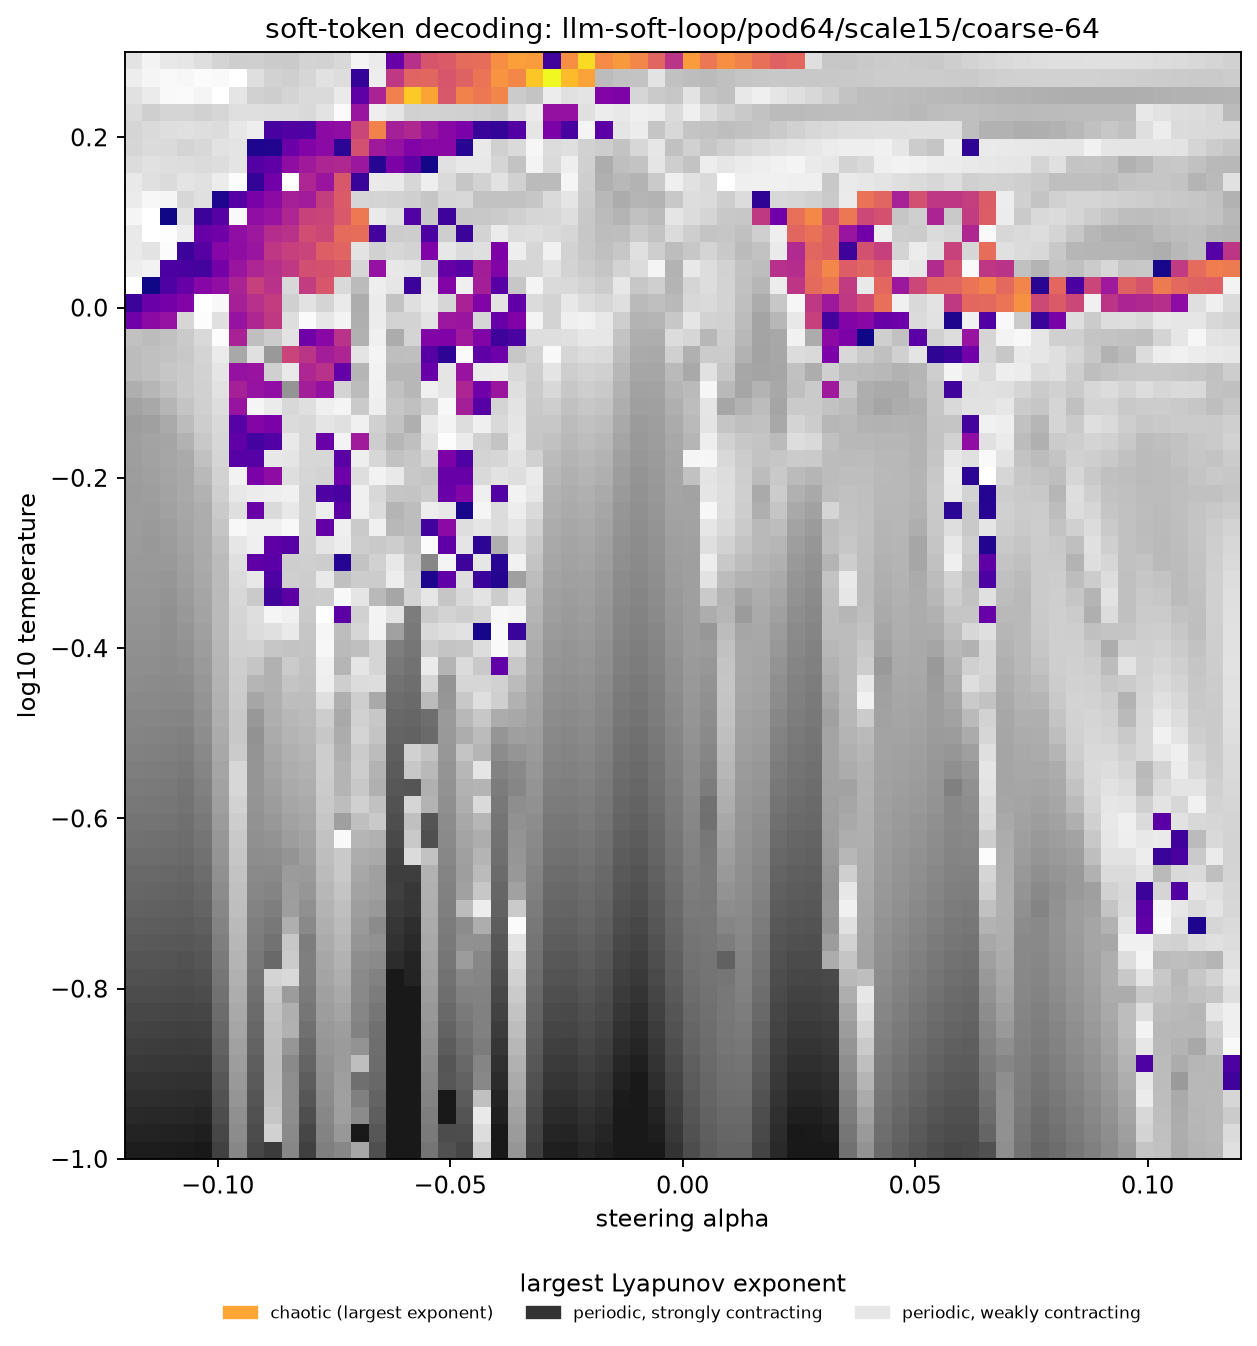
\includegraphics[width=0.55\linewidth]{fig-qwen15-coarse.png}
\caption{Qwen2.5-1.5B soft-token map, coarse $64^2$ float64 cells, rendered as Figure~\ref{fig:stripes} (left).}
\label{fig:qwen15}
\end{figure}

\section{A second system: recurrent depth}
\label{sec:huginn}
Huginn-0125 iterates a recurrent block at fixed input tokens \cite{geiping2025recurrent}. For a
GSM8K-style prompt the native loop converges to a fixed point whose leading Jacobian pair is $0.588\pm0.771i$
(modulus $0.970$). For the relaxed loop $h\leftarrow(1-\lambda)h+\lambda F(h)$ this predicts a Neimark--Sacker
bifurcation at $\lambda_c=2(1-\operatorname{Re}\mu)/|1-\mu|^2=1.0777$. The latent state decays below it and settles on
a closed curve above it; a fit of the squared amplitude gives $\lambda_c=1.0778$, with
$A/\sqrt{\lambda-\lambda_c}=0.52$--$0.54$ (supercritical) and a rotation of 0.156 turns per step. Causal attention
makes the loop block lower-triangular in token positions; the first position to oscillate is the ``.'' of the
prompt, and all later positions follow. Fixed-point and Jacobian stability of looped models has been studied
before \cite{yang2026stars}; the predicted crossing and its amplitude law are what this adds.
\inprogress{rotation number on the invariant circle (quasi-periodic or locked).}
\planned{causal clamp of the first unstable position on held-out prompts.}

\section{Discussion}
\label{sec:discussion}
\paragraph{What is and is not claimed.} The objects here are invariant sets and bifurcations of an exactly defined
smooth map built from a frozen model's own computation. The phenomena are classical in nonlinear dynamics
\cite{pomeau1980intermittent,gallas1993structure,facanha2013endoskeletons,vitolo2011hubs}; what is new is their
quantitative realization inside a pretrained language model, and the use of numerical continuation and normal
forms on such a model. We do not claim that ordinary sampled generation is chaotic in this sense
(Section~\ref{sec:bridge}), nor that the shapes in the maps are shrimps beyond the verified cusps.
\paragraph{Limitations.} One model family so far at full resolution, one prompt, one steering construction; a
constructed one-token-window system; numerical validation, not proof.
\planned{discussion of what the bifurcation structure means for repetition, steering discontinuities and safe
operating regions of inference-time control.}

\section{Evidence and reproducibility}
\label{sec:evidence}
We label claims by an evidence ladder: rung 1, numerically validated (tolerances, residuals, convergence,
precision varied); rung 2, cross-checked (independent estimate, implementation or hardware); rung 3,
computer-assisted proof. The normal-form coefficient $ab$ is at rung 2 (derivatives against stable-branch
multipliers); passage predictions, orbits, curves and cusps are at rung 1.
\planned{independent reimplementation (Codex task 2) to raise orbits and the normal form to rung 2; interval
proof of the period-8 orbit (Codex task 1) for rung 3.}
Code: \texttt{tools/explore\_llm\_soft\_loop.py}, \texttt{tools/bifurcation\_curves.py},
\texttt{tools/explore\_latent\_loop.py}; raw data hash receipts in
\texttt{evidence/llm-dynamics-data-receipts.json}. \planned{public code and data release at submission.}

\bibliographystyle{unsrtnat}
\bibliography{references}
\end{document}
